\documentclass{beamer}

\usepackage{cmap}
\usepackage[english,russian]{babel} % add eng,rus(base) package
\usepackage[T1,T2A]{fontenc}        % add eng,rus encoding support
\usepackage[utf8]{inputenc}         % add UTF8 support

% Use it for English document
%\usepackage[utf8]{inputenc} % add UTF8 support
%\usepackage{fontspec}       % to use any font known to the operating system
%\setmainfont{PT Serif}      % set defolt font

\usepackage{amsmath, amsfonts, amssymb, amsthm, mathtools} % add math support

\linespread{1}               % length between str
\setlength{\parindent}{16pt} % red str
\setlength{\parskip}{6pt}   % length between paragraphs

\usepackage[backend=biber, style=authoryear-icomp]{biblatex}
\addbibresource{$HOME/latex-templates/biblio.bib}            % path to bibliography base

\usetheme{Madrid}
\setbeamertemplate{frametitle}[default][center]

\renewcommand{\thefootnote}{\arabic{footnote}}
 % here is document's settings for russian
%\input{$HOME/studyproject/universe/history/preamble-beamer-eng.tex} % here is document's settings for english


\title{Иван III --- Первый государь всея Руси}
\author{Немков Н.М.}
\institute[МГТУ]{МГТУ им. Н.Э. Баумана}
\date{09.10.2023}
\logo{
\includegraphics[width=1cm]{images/logo}}

\begin{document}

\begin{frame}
\maketitle
\end{frame}




\begin{frame}{Иван III}
	\begin{columns}
		\begin{column}{0.45\textwidth}

			Иван III (1440-1505) выдающийся правитель который создал единое Русское государство.

		\end{column}

		\begin{column}{0.45\textwidth}

			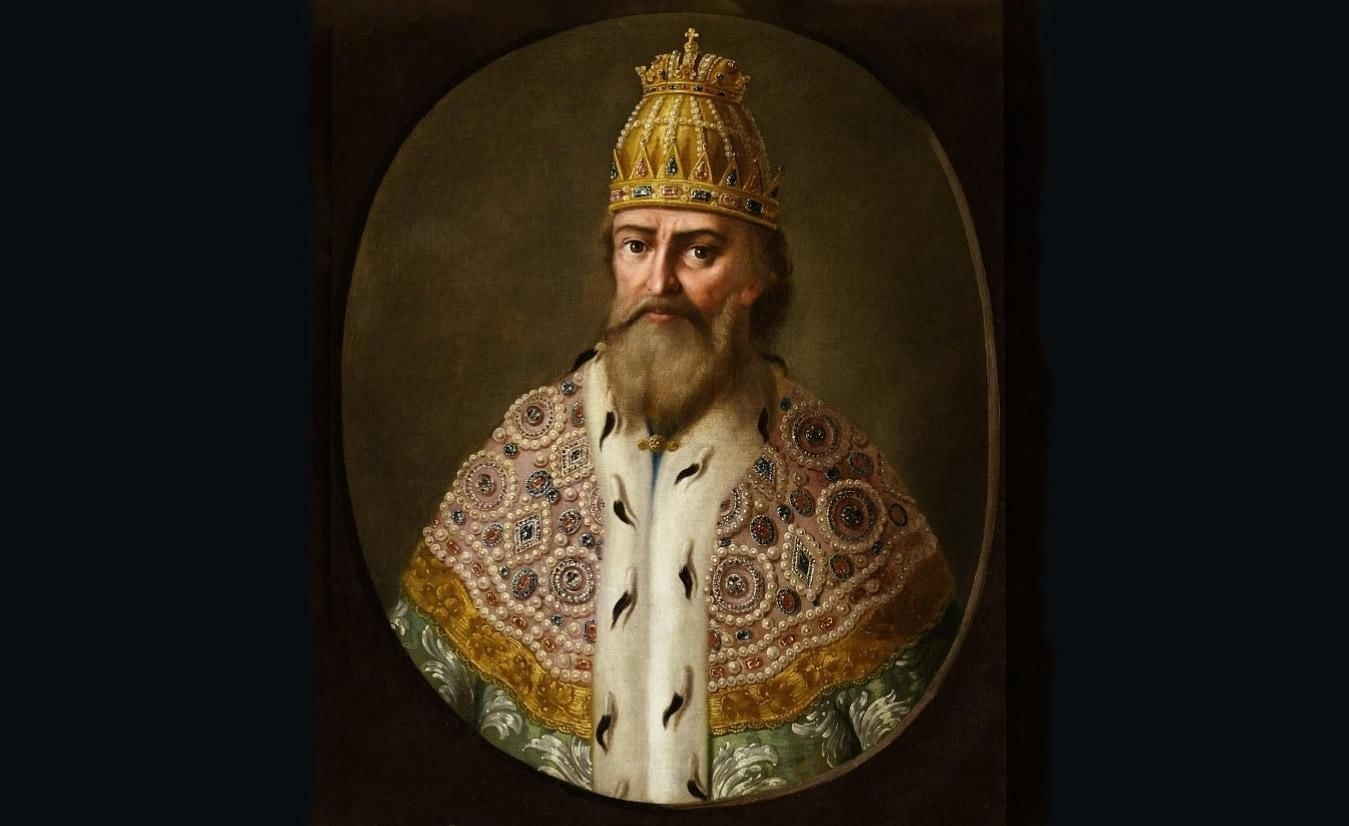
\includegraphics[width=1\textwidth]{images/ivan-1}

		\end{column}
	\end{columns}
\end{frame}

\begin{frame}{}

	Одним из его самых величайших достижений стало присоединение(подчинение) Новгорода.

\end{frame}

\begin{frame}{}
	Первый шаг по присоединению Новгорода сделал еще Василий Темный.

	1456г был подписан яжелбитский мир между Москвой и Новгородом по условиям которого Новгород лишался самостоятельной внешней политики.
\end{frame}

\begin{frame}{Первый поход на Новгород}
	Второй шаг сделал Иван III. И это был знаменитый поход на Новгород 1471г.

	Иван пошел вместе со своим войском. Было несколько стычек в том числе и на реке Шелонь 14 июля 1471г.

	Командывал московскими полками Данил Дмитриевич Холмский.

	Новгородское войско было разбито после чего они начали переговоры.
\end{frame}

\begin{frame}
	По результатам переговоров Иван оставил Новгороду систему управления но основные решения Новгород будет принимать только соглосовав их с Москвой.
\end{frame}

\begin{frame}{Религиозная война}
	Иван III был не только прекрасным дипломатом но и большим мастером в социальной димогогии.
\end{frame}

\begin{frame}{}
	Еще одна тонкость войны за Новгород это то что Иван III хотел представить себя как справедливый судья.
\end{frame}

\begin{frame}{}
	В итоге к нему обращалось очень много бедняков которых обидели Новгородские баяре. Судил он в сторону простых людей что бы завоевать доверие.
\end{frame}

\begin{frame}{Второй поход на Новгород}
	\begin{columns}
		\begin{column}{0.45\textwidth}

			В результате второго похода на Новгород они признали себя побежденными. Иван приказал снять вечевой колокол.

		\end{column}

		\begin{column}{0.45\textwidth}
			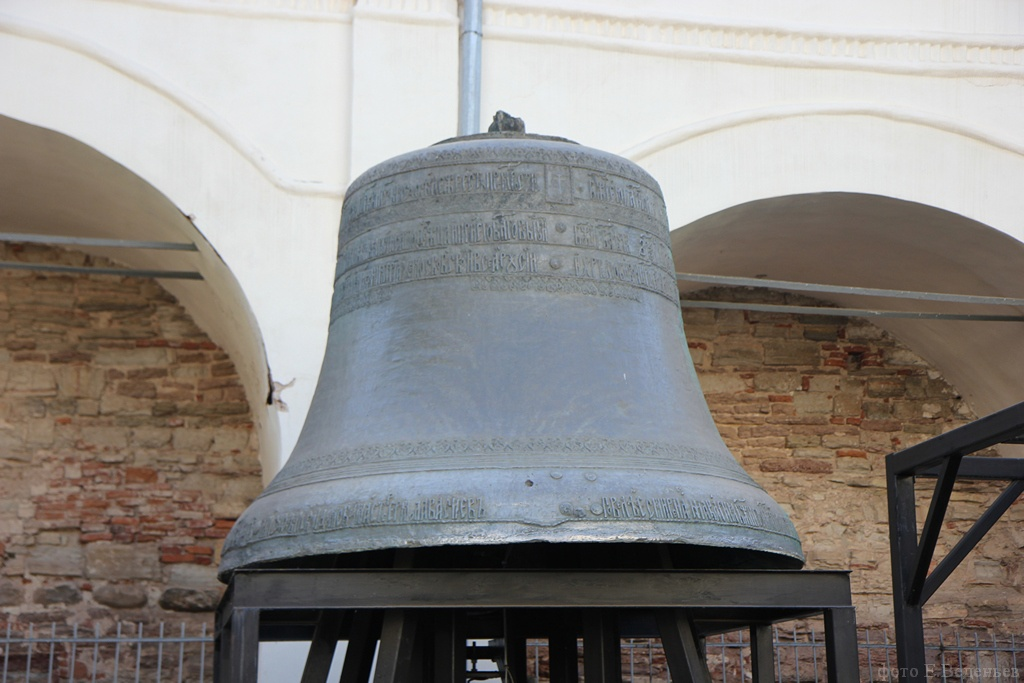
\includegraphics[width=0.9\textwidth]{images/ivan-2}
		\end{column}
	\end{columns}
\end{frame}

\begin{frame}{}

	Впредь Новгородская политическая система анулировалась и Новгород оставался провинцией Московского государства.

	Им управляли Московские Дьяки.
\end{frame}
\begin{frame}{Выгода}
	Присоединив Новгород Иван получил огромный финансовый потенциал
\end{frame}
\begin{frame}{}
	Следующим шагом Ивана было объединение с Тверью 1485г

	В итоге Тверь вошла в Московское государство без кровопролития
\end{frame}
\begin{frame}{}
	Последним крупным успехом Ивана III было присединение Вятки

	Он хотел использовать ее как плацдарм для нападения на Казань
\end{frame}

\section{Благоданость}
\begin{frame}
	\centering
	\huge
	Спасибо за внимание!
\end{frame}


\end{document}
